\documentclass[../../szobeli.tex]{subfiles}

\begin{document}

    \begin{center}
        \noindent\fbox{%
            \parbox{160mm}{
                \textbf{Minimális költségű feszítőfa}, mkffák struktúrája, \textbf{Kruskal-algoritmus} \underline{helyessége}, villamos hálózathoz tartozó normál fa keresése.
            }
        }
    \end{center}

    \begin{itemize}
        \item \textbf{Minimális költségű feszítőfa:} Adott a $G = (V,E)$ irányítatlan gráf élein a $k:E \rightarrow \mathbb{R}^+$ költségfüggvény. Az $F \subseteq E$ élhalmaz \textcolor{red}{költsége} az $F$-beli élek összköltsége: $k(F) = \sum_{f\in F}k(F)$. \\ Az $F \subseteq E$ élhalmaz $G$-ben \textcolor{red}{minimális költségű feszítőfa} (\textcolor{red}{mkffa}), ha \begin{itemize}
            \item[(1)] $(V,F)$ a $G$ feszítőfája, és
            \item[(2)] $k(F) \leq k(F')$ teljesül a $G$ bármely $(V,F')$ feszítőfájára. (akkor mkffa ha ennek a feszítőfának a legkisebb a költsége az összes többi feszítőfa közül)
        \end{itemize}
        \begin{equation*}
            F_i :=\begin{cases}
                F_{i-1}\cup \{e_i\} & \text{ha $F_{i-1}\cup \{e_i\}$ körmentes.} \\
                F_{i-1} & \text{ha $F_{i-1}\cup \{e_i\}$ tartalmaz kört. \;\;\; $F:=F_m$}
            \end{cases}
        \end{equation*}

        (1 eset) az élt bevesszük a ffába, ha az nem alkotna kört 
        
        (2 eset) ha az él bevételével kör keletkezne, nem vesszük be a ffa-ba

        \item \textbf{Minimális költségű feszítőfa:} olyan $F\in E$ élhalmaz, amire $(V,F)$ fa, és $k(F)$ minimális.
        \item Mkkfák struktúrája: $G=(V,E)$ gráf és $k:E \rightarrow \mathbb{R}^+$ költségfüggvény esetén legyen $G_c$ a legfeljebb $c$ költségű élek alkotta feszítő részgráfja $G$-nak: $G_c = (V,E_c)$, ahol $E_c := \{e \in E : k(e)\leq c\}$. \\ \textbf{Megf:} A $G$ gráfon futtotott Kruskal-algoritmus outputja tartalmazza $G_c$ egy feszítő erdejét minden $c \geq 0$ esetén. \\ \textbf{Lemma:} Tfh $F=\{f_1,f_2,\dots,f_l\}, k(f_1) \leq k(f_2) \leq \dots \leq k(f_l)$ és $F\cap E_c$ a $G_c$ egy feszítő erdeje $\forall c \geq 0$-ra. Tfh $F' = \{f'_1, f'_2,\dots,f'_l\}$ a $G$ egy feszítő erdejének élei, és $k(f'_1) \leq k(f'_2) \leq \dots \leq k(f'_l)$. Ekkor $k(f_i) \leq k(f'_i)$ teljesül $\forall 1 \leq i \leq l$ esetén, így $k(F) \leq k(F')$. \\ \textbf{Köv:} (1) A Kruskal-algoritmus outputja a $G$ gráf egy minimális költségű feszítő erdeje. \\ \textbf{Köv:} (2) Az $F'$ élhalmaz pontosan akkor minimális költségű feszítő erdeje $G$-nek, ha $F' \cap E_c$ a $G_c$ egy feszítő erdeje minden $c \leq 0$-ra. \\ \textbf{Biz:} A Lemma bizonyítja az elégségességet.
        \item \textbf{Kruskal algoritmus:} \begin{itemize}
            \item \underline{Input:} $G=(V,E)$ gráf, és $k:E\rightarrow \mathbb{R}^+$ költségfüggvény.
            \item \underline{Output:} minimális költségű feszítőfa.
            \item \underline{Működés:} minden lépésben megépítjuk a legolcsóbb élt, ami nem hoz létre kört. Mohó algoritmus, mert csak azzal törődik, ami éppen a legalacsonyabb költségű. Az így keletkezett fa a $G$ gráf egy minimális költségű (súlyú) feszítőfája.
            \item \underline{Helyességének bizonyítása:} tegyük fel, hogy az algoritmus helytelen, ekkor létezik egy $f$ él, amit $e$ helyére bevéve olcsóbb feszítőfát kapunk. Ekkor azonban $f$ költsége kisebb, mint $e$ költsége, így $f$-et az algoritmussal korábban már ellenőriztük, tehát ellentmondásra jutottunk, azaz a feszítőfa minimális költségű.
        \end{itemize}
        \item Villamos hálózatohoz tartozó normál fa keresése: \\ 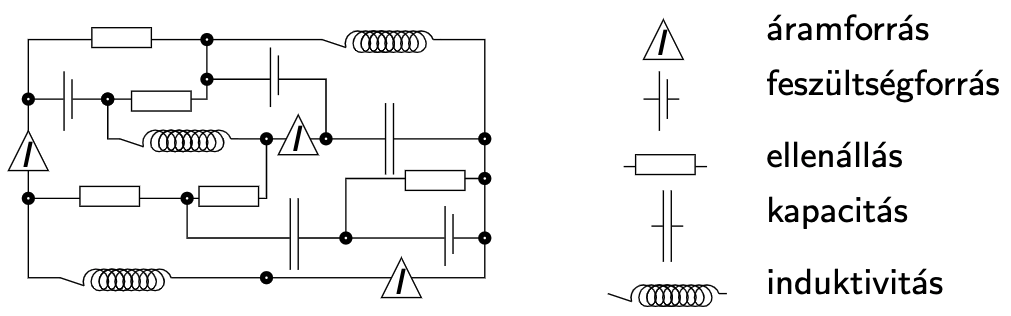
\includegraphics[scale=0.45]{./img/1.png} \begin{itemize}
            \item Tegyük fel, hogy egy áramkör a fenti kétpólusú áramköri elemekből áll. Az áramkör tulajdonképpen egy gráf, aminek minden éle egy-egy áramköri elemnek felel meg. Az, hogy mi történik (mik lesznek az élek mentén az áramerősségek, és a gráfcsúcsok között a potenciálkülönbségek), a Kirchoff- ill. Ohm-törvényekkel írható le.
            \item \textbf{Csomóponti törvény:} a gráf egy ponthalmazából kilépő éleken az áramerősségek előjeles összege 0.
            \item \textbf{Huroktörvény:} a gráf tetszőleges köre mentén a potenciálkülönbségek összege 0.
            \item Mikor "értelmes" egy ilyen hálózat? Akkor, ha a fenti törvényekkel felírt egyenletrendszer egyértelműen megoldható. Bizonyítható, hogy ha a fenti esetek egyike sem áll fenn, akkor a megoldás egyértelmű, a hálózat "értelmes". Ennek a a bizonyítéka a \textcolor{red}{normál fa}: $G$ olyan feszítőfája, ami minden feszültségforrást tartalmaz, de egyetelen árramforrást sem (és mindemellett a legtöbb kapacitást és a lehető legkevesebb induktivitás tartalmazza).
            \item \textbf{Normál fa keresése:} fesz.forrás (1), kapacitás (2), ellenállás (3), induktivitás (4), áramforrás (5) élköltségekhez keressünk mkffát! Ha ez tartalmaz áramforrást, vagy nem tartalmaz minden feszültségforrást, akkor nincs normál fa, egyébként a mkffa egy normál fa és egyértelmű a megoldás "értelmes" a hálózat.
        \end{itemize}
    \end{itemize}
    
\end{document}